\documentclass{article}

\usepackage{cite}
\usepackage{graphicx}

\title{Final Project Literature Review}
\author{Christian Ulfert}
\date{\today}

\begin{document}

\maketitle

\tableofcontents    

\section{Existing work}
\subsection{Tetris}
\paragraph{Introduction}
Tetris is one of the most popular games in the history of computer gaming. Developed in 1984 by Alexey Pajitnov, as a testbed for emerging computing hardware it has trancended its initial purpose and become a cultural icon. 
After initial struggles to leave the UDSSR the big break came when Nintendo bundled it with the original Gameboy in 1989. 
Through capturing a whole generation of newly computer-affine people it has cemented its place in gaming history. The total estimated sales of Tetris are over 500 million copies, most of them in digital form, which only came reality 3 decades after the inital game was developed.
It has also captured the imagination of countless scientists and mathematicians, who have studied the game from a variety of perspectives (computer science, psychology, medicine, mathematics...).
\paragraph{Gameplay}
The staple of tetris is the tetrominoe. A collection of 4 squares arranged in different shapes. The tetrominoes fall from the top of the screen into a 10x20 playing field, they can not be stopped. The player rotates and moves these shapes to arrange them at the bottom of the playing field in a way such they cover a whole row. A full row will be removed from the playing field, giving the player more room to place blocks, and changing the arrangement of the blocks, potentially opening new positions for the next blocks.
In addition the player receives a score for each row removed. The score is higher for removing multiple rows at once. The game ends when the playing field is full and no more blocks can be placed.
\begin{figure}
    \label{fig:poly}
    \centering
    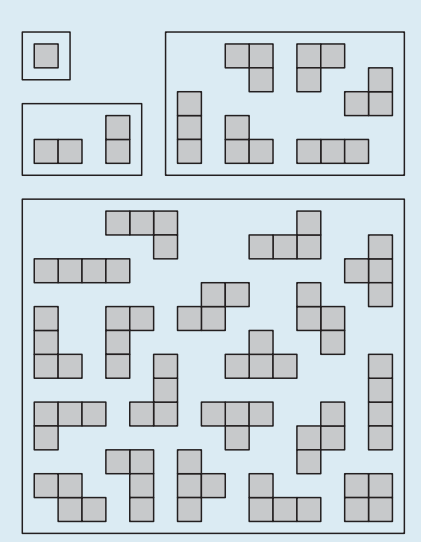
\includegraphics[width=0.6\textwidth]{polynominoes.png}
    \caption{The single monomino (A(1) = 1),
    the two dominoes (A(2) = 2), the A(3) = 6
    triominoes, and the A(4) = 19 tetrominoes
    (Tetris pieces) \cite{polyominoes}}  
\end{figure}
Tetrominoes are a special case of polyominoes (A(4)), which are shapes made up of squares. This is another interesting field of study, and a possible route to increase complexity in tetris, as the number of possible shapes increases dramatically as discussed in Barequet et al.\cite{polyominoes} and visualized in Figure \ref{fig:poly}.
This path however will not be followed in this project.

\subsection{Frac 4D}
\subsection{4DTris}

\section{Literature}
\subsection{}


\section{Algorithms}
\subsection{}


\bibliographystyle{acm}
\bibliography{references}

\end{document}